\documentclass{beamer}
\usepackage{relsize}
\usepackage{color}

\usepackage{listings}
\usetheme{CambridgeUS}
%\usepackage{beamerthemesplit} % new
\usepackage{enumitem}
\usepackage{amsmath}                    % See geometry.pdf to learn the layout options.
\usepackage{amsthm}                   % See geometry.pdf to learn the layout options. There
\usepackage{amssymb}                    % See geometry.pdf to learn the layout options.
\usepackage[utf8]{inputenc}
\usepackage{graphicx}
\usepackage[english,bulgarian]{babel}
\usepackage{tikz}


\usepackage{caption}

\usetheme{CambridgeUS}
\usecolortheme{crane}

\lstset{language=C++,
                basicstyle=\ttfamily,
                keywordstyle=\color{blue}\ttfamily,
                stringstyle=\color{red}\ttfamily,
                commentstyle=\color{green}\ttfamily,
                morecomment=[l][\color{magenta}]{\#}
}

\newtheorem{mydef}{Дефиниция}[section]
\newtheorem{lem}{Лема}[section]
\newtheorem{thm}{Твърдение}[section]

\DeclareMathOperator{\restrict}{\upharpoonright}

\setitemize{label=\usebeamerfont*{itemize item}%
  \usebeamercolor[fg]{itemize item}
  \usebeamertemplate{itemize item}}

\setbeamercovered{transparent}

\captionsetup{font=tiny} 

\begin{document}
\title[Увод в курса]{Въведение във функционалното програмиране}
\frame{\titlepage}

\section{Увод}
\subsection{Императивно vs. функционално програмиране}

\frame{\frametitle{Von Neumann архитектура}

\begin{figure}
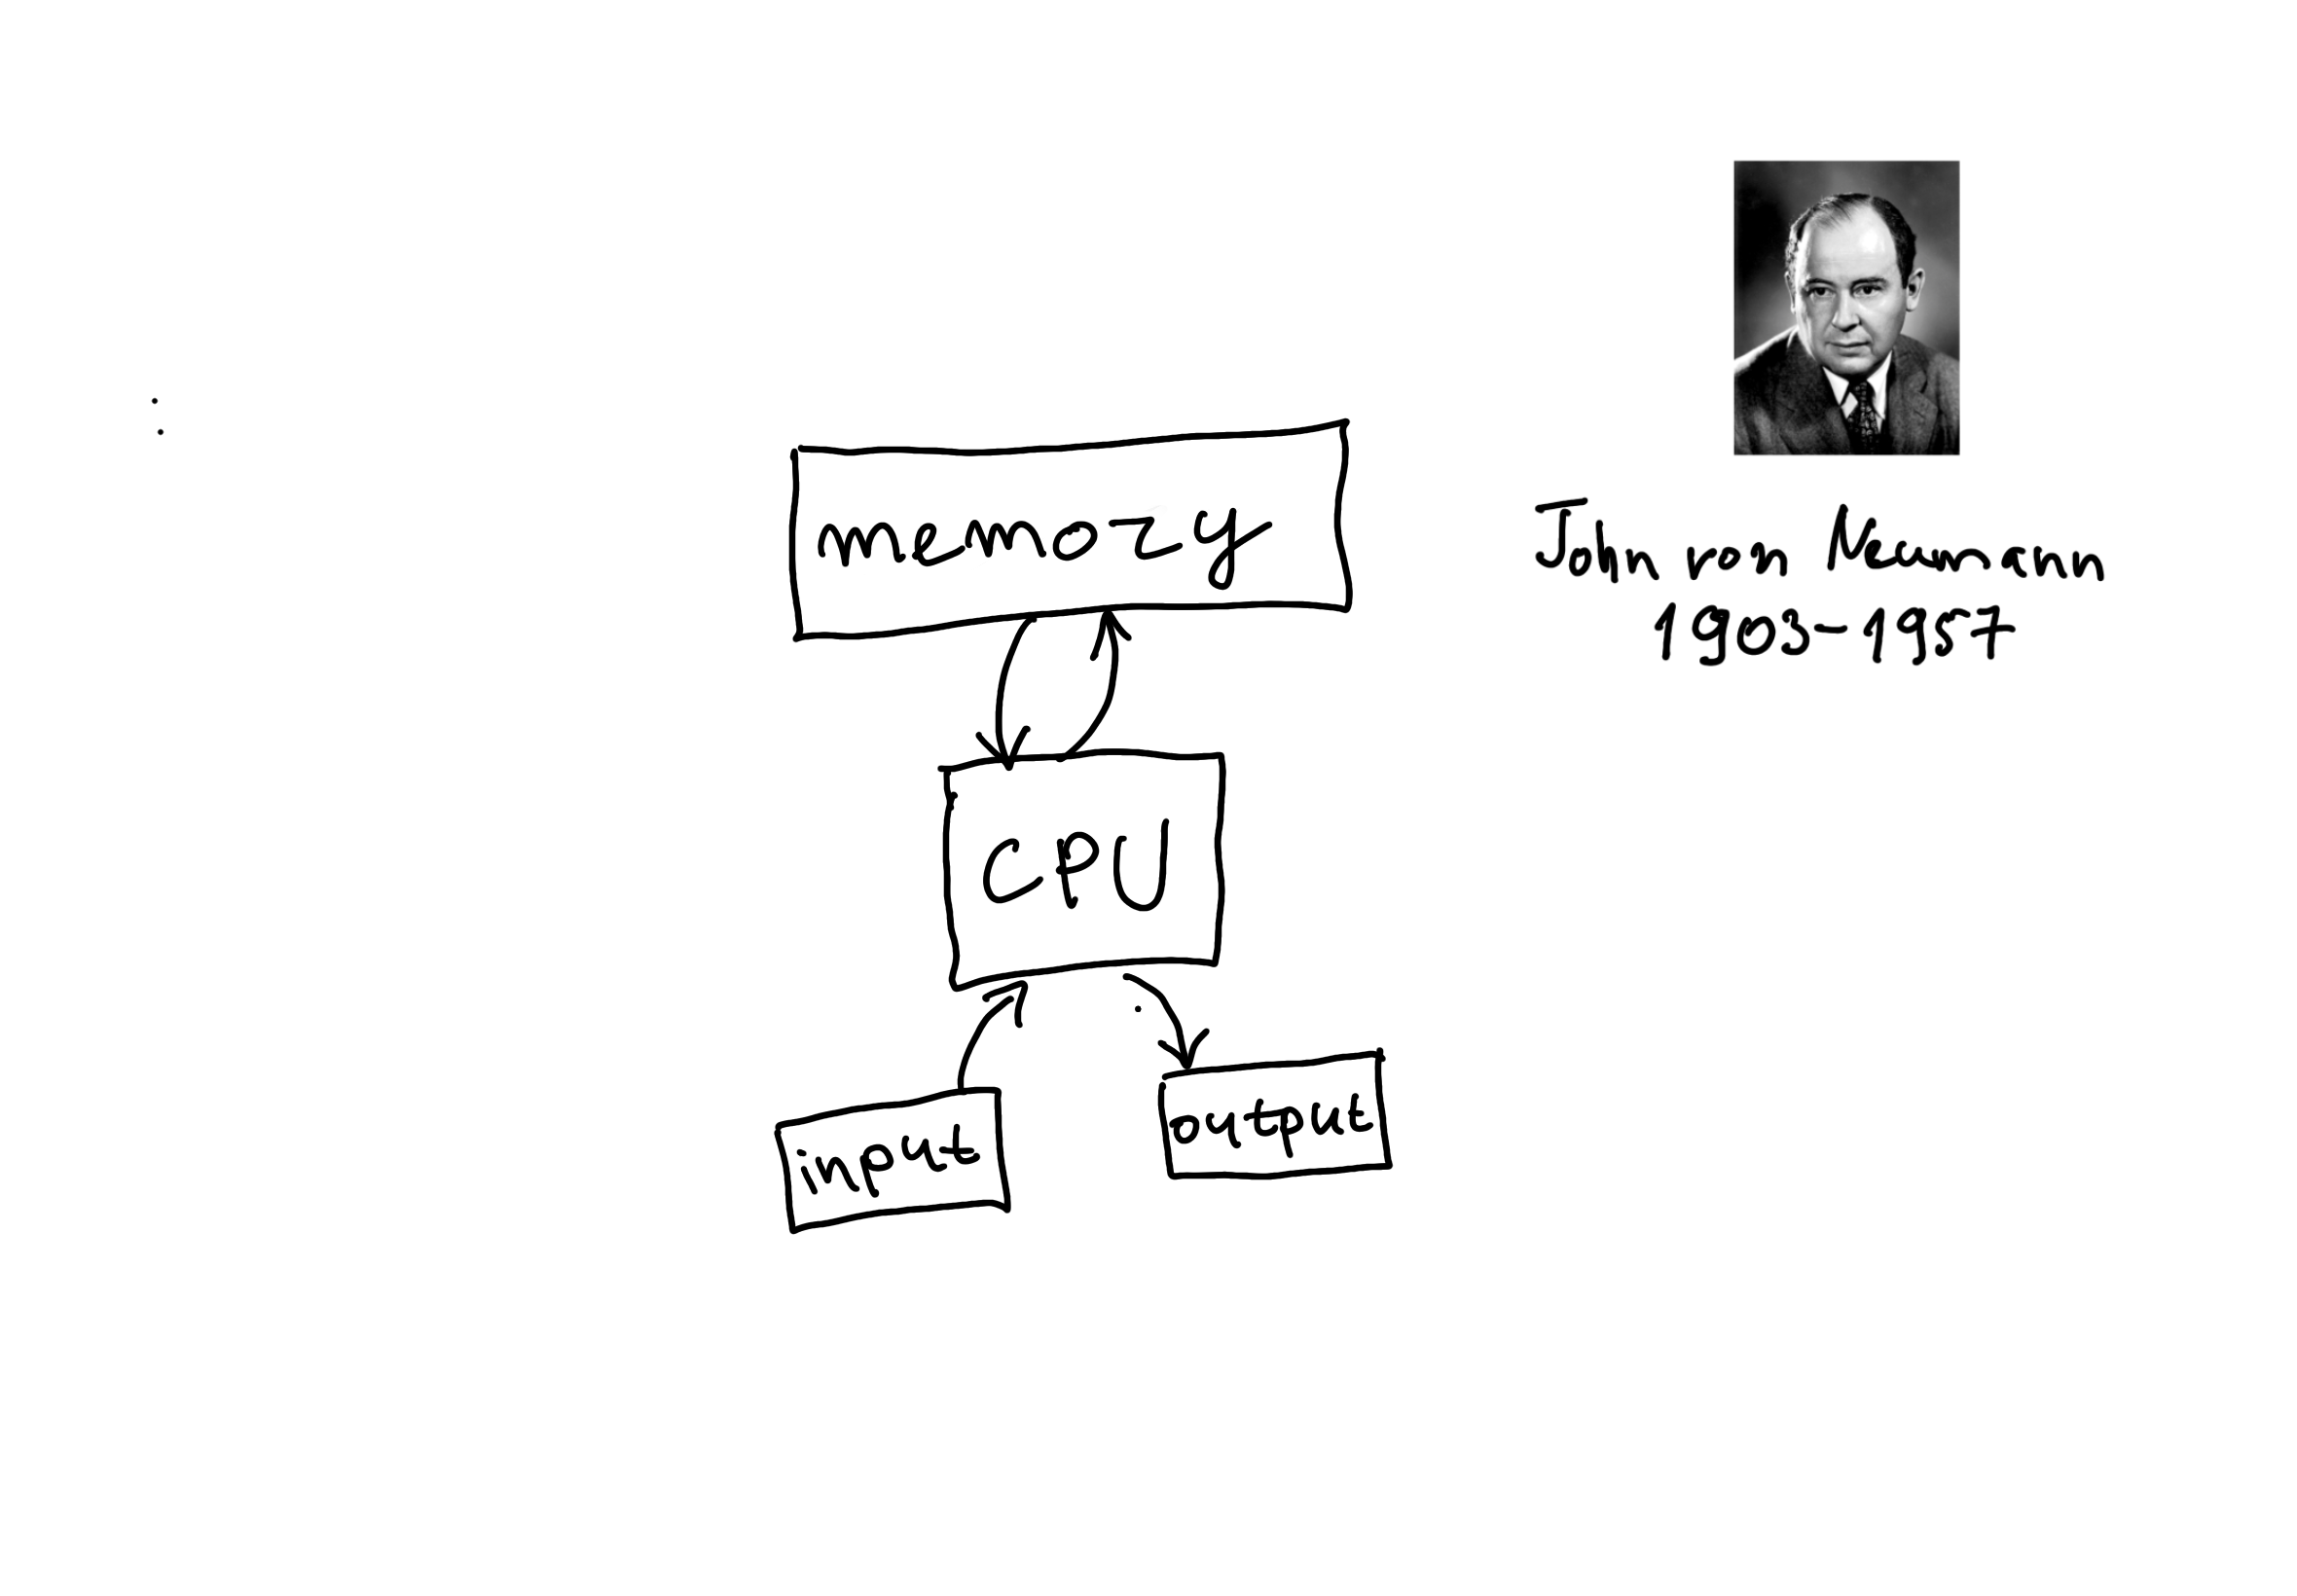
\includegraphics[width=12cm]{images/von-neumann}
\end{figure}

}

\frame{\frametitle{Императивен стил}

\begin{figure}
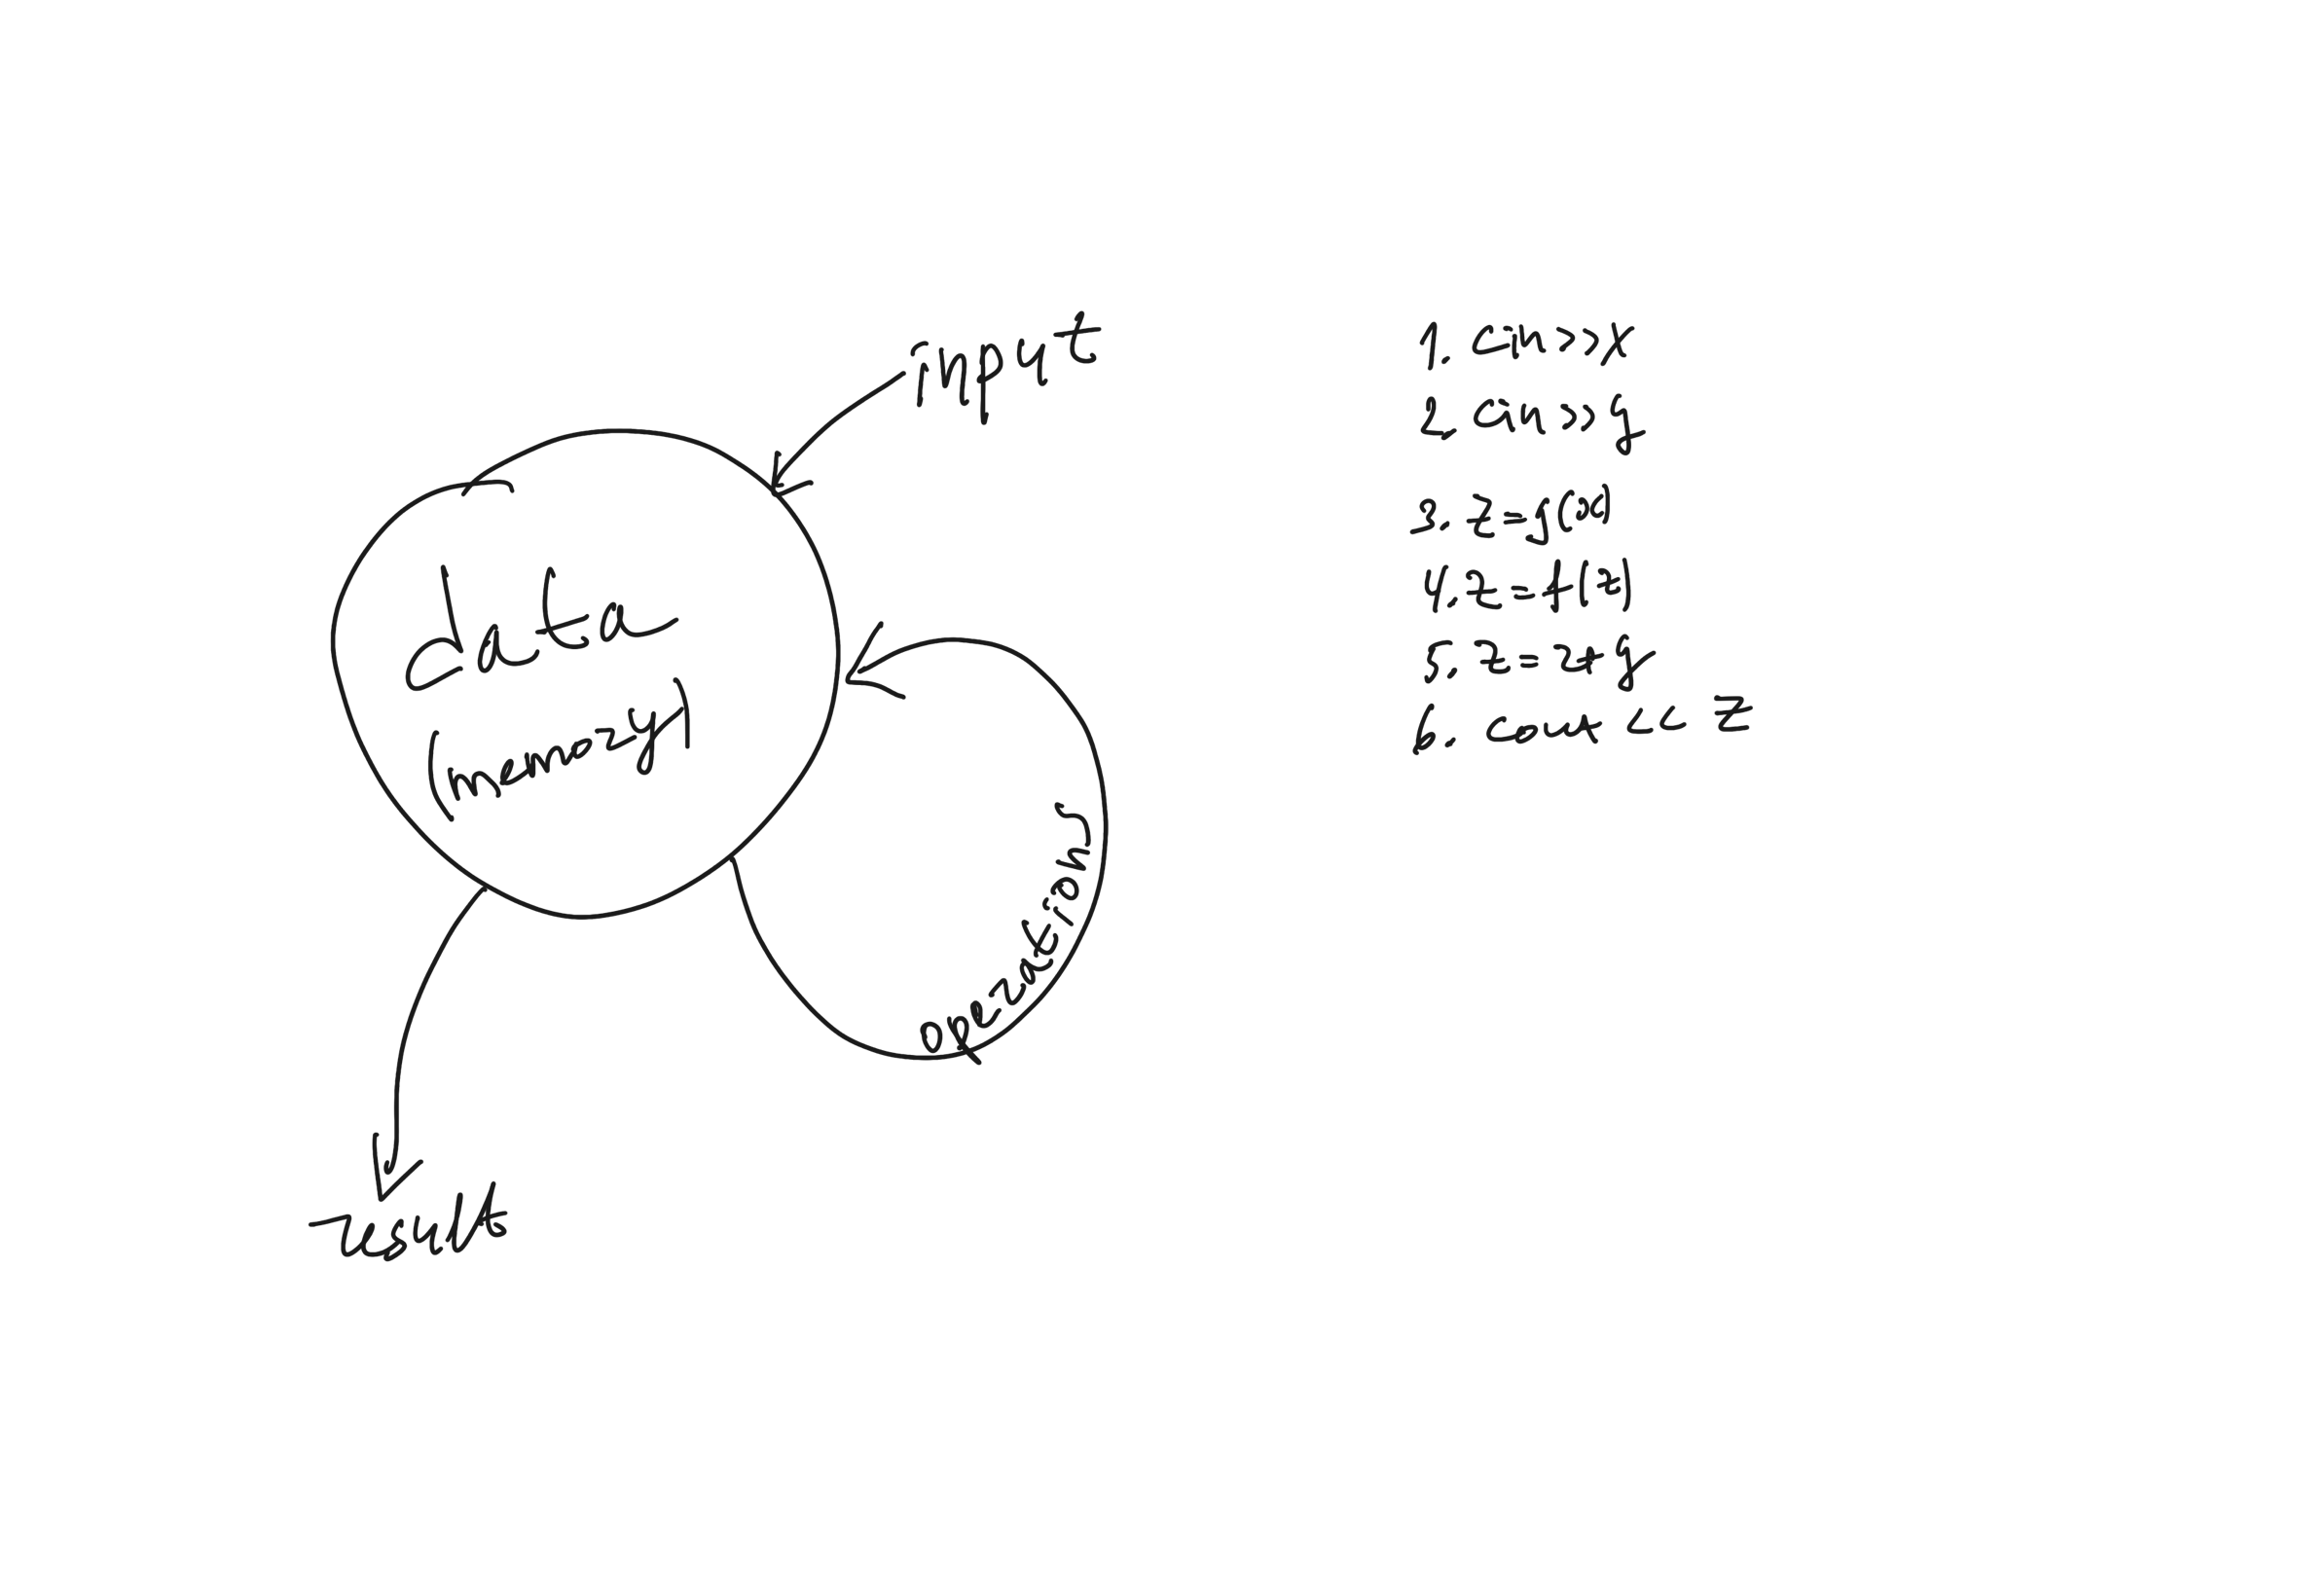
\includegraphics[width=12cm]{images/data-operations}
\end{figure}

}


\frame{\frametitle{Функционален стил}

\begin{figure}
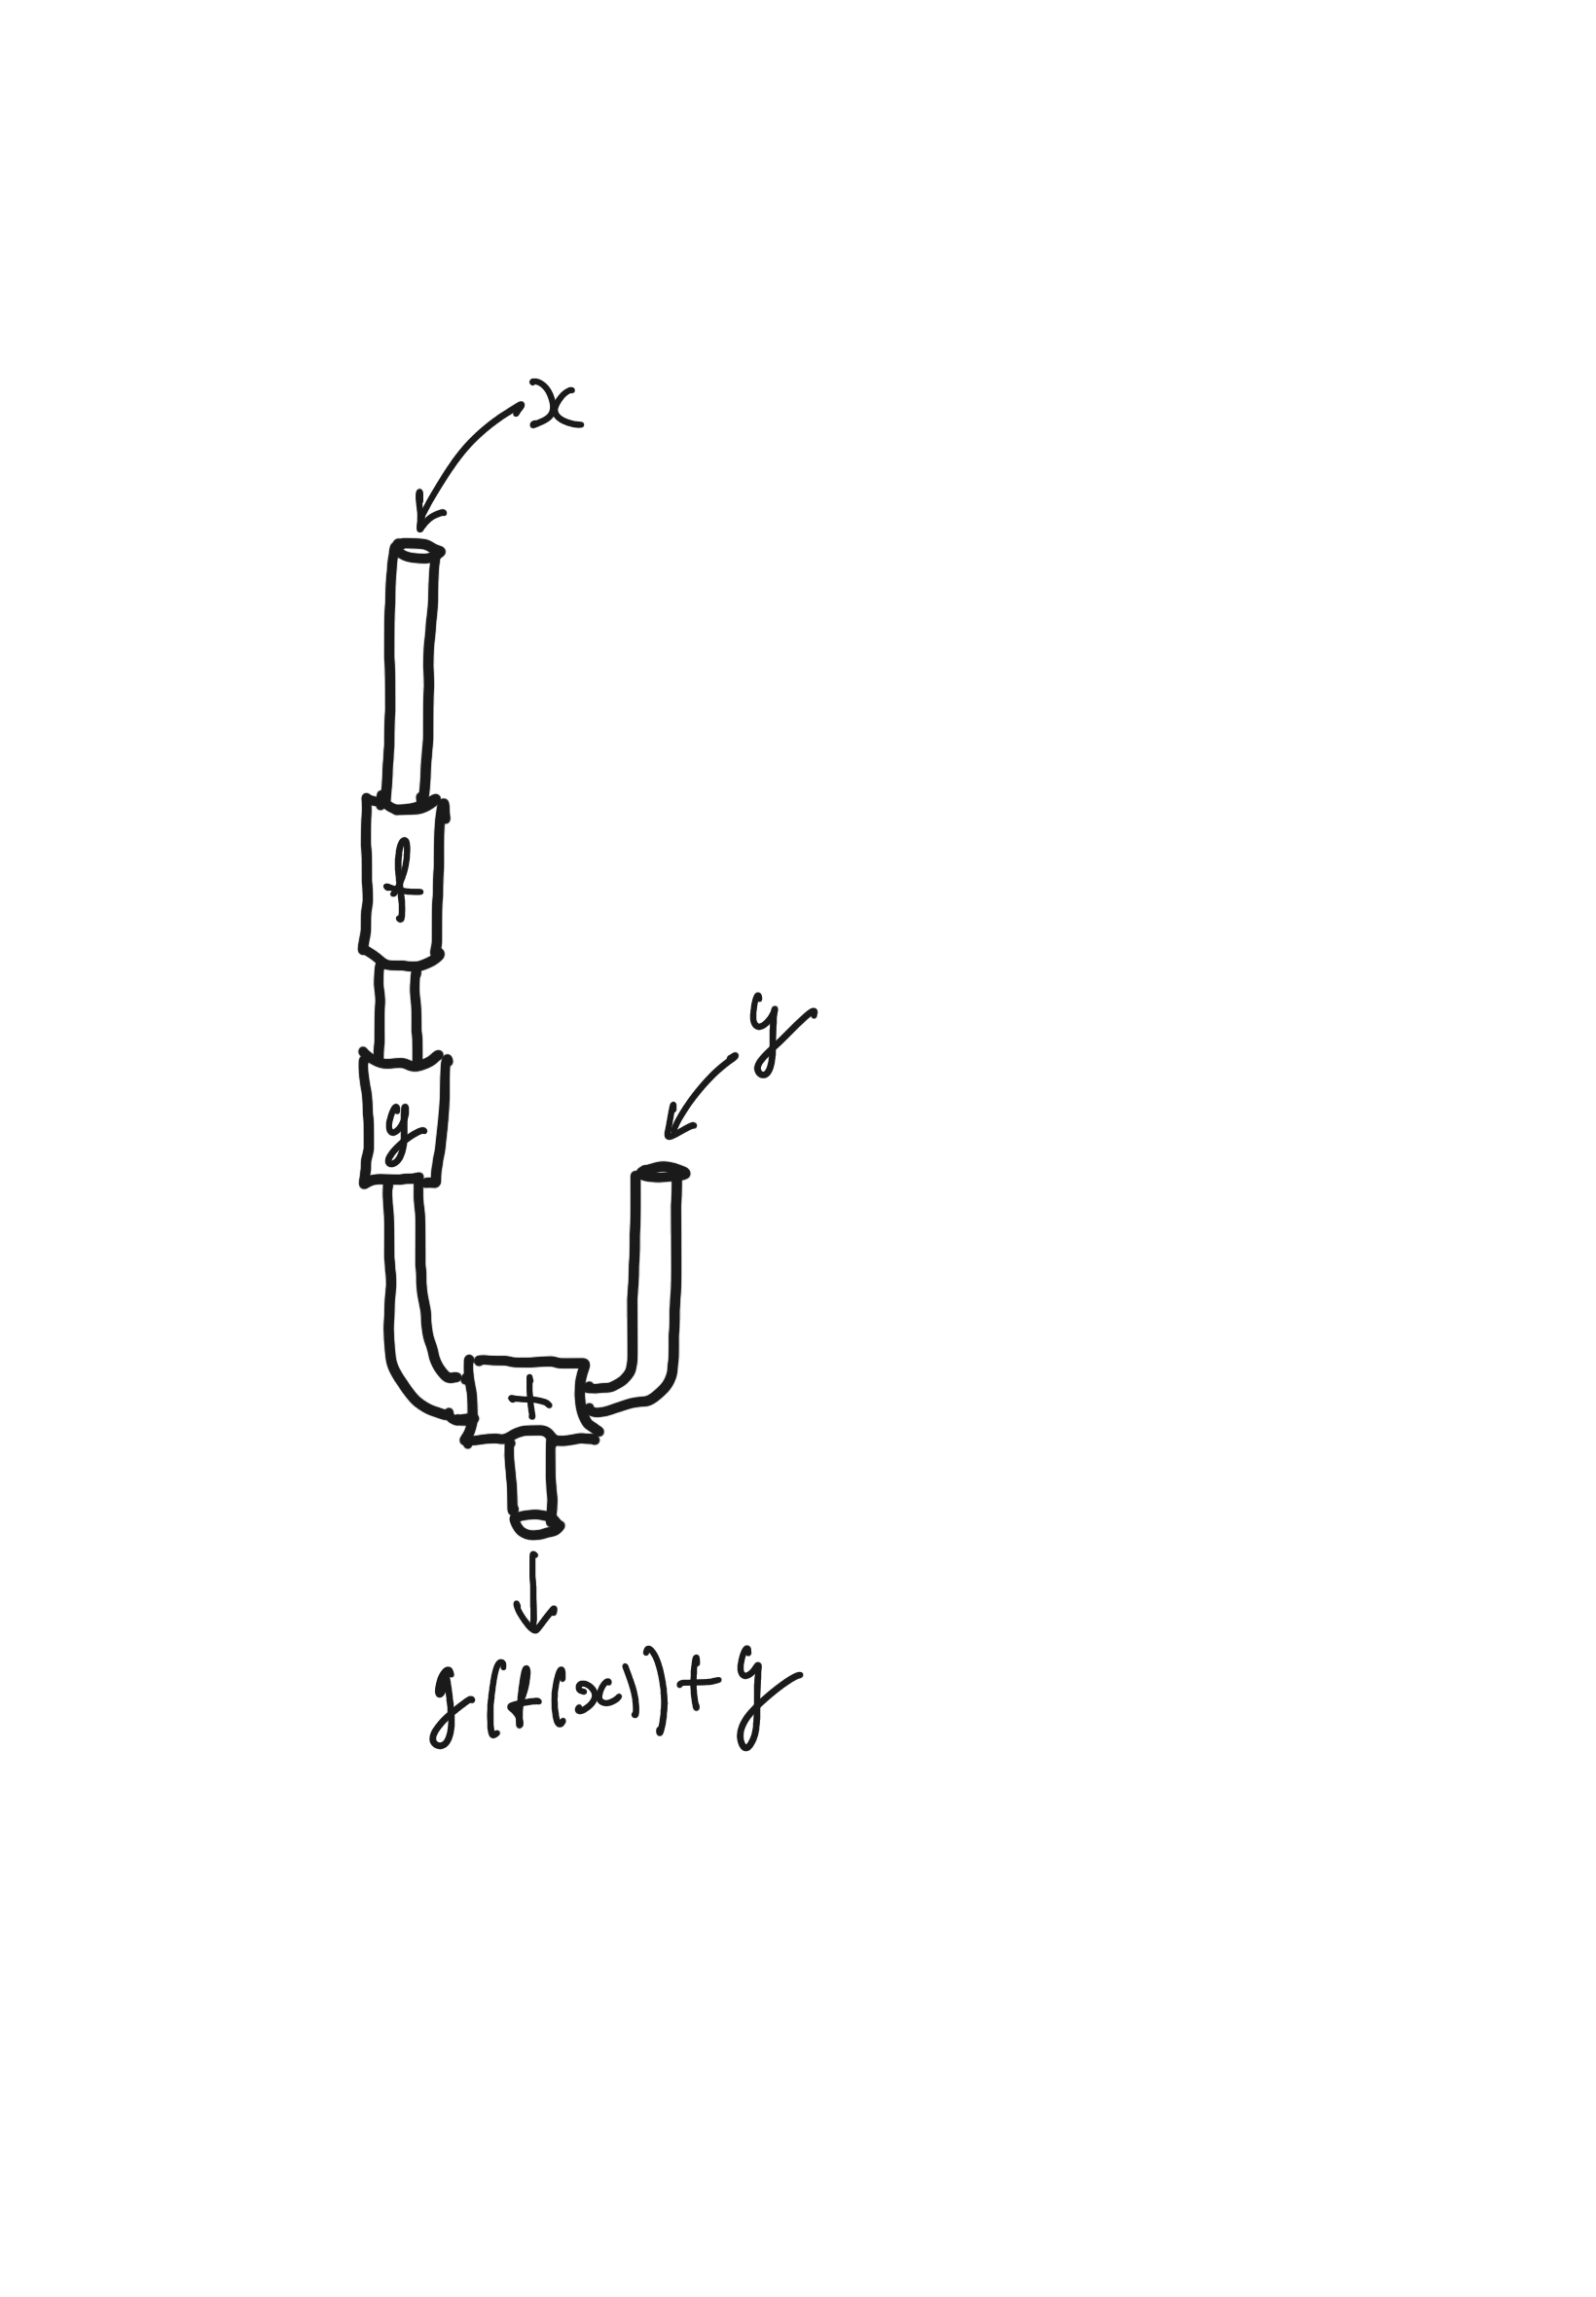
\includegraphics[width=6cm]{images/pipes}
\end{figure}

}

\frame{\frametitle{Сравнение}

\begin{figure}
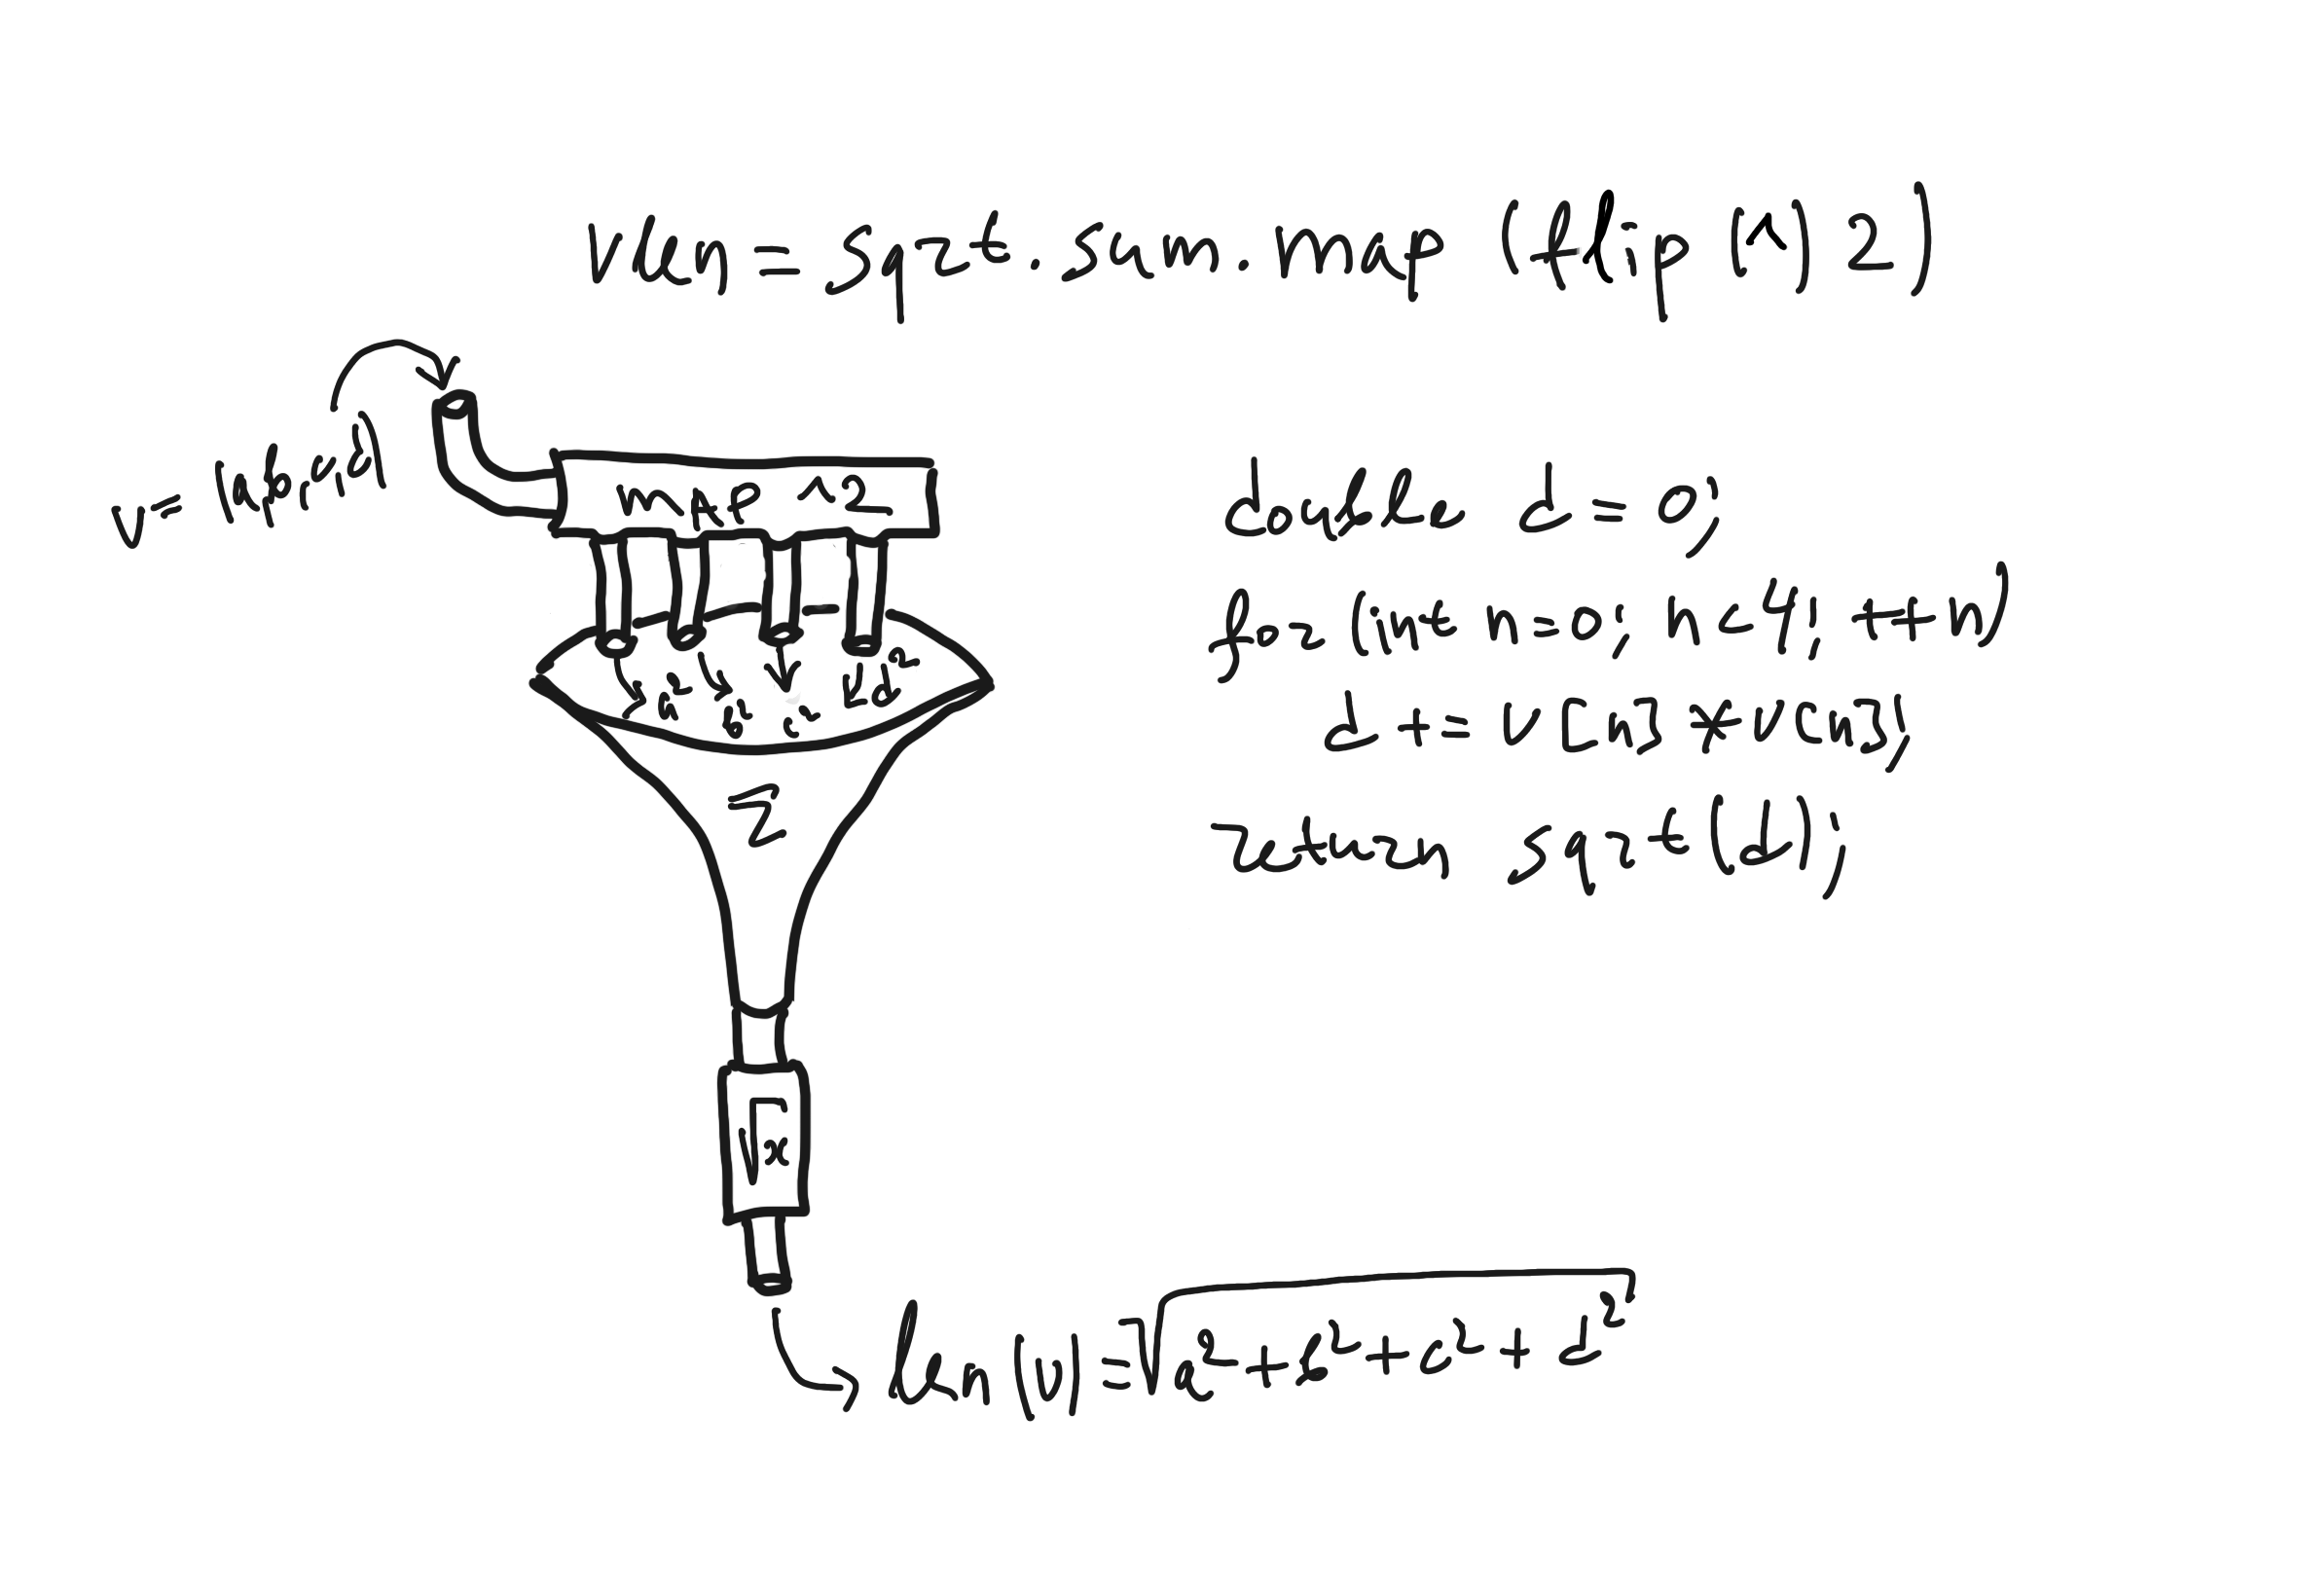
\includegraphics[width=12cm]{images/vlen}
\end{figure}

}

\section{Език за програмиране Haskell}

\begin{frame}
  \centerline{Език за програмиране Haskell}
\end{frame}


\subsection{}

\begin{frame}[fragile]
  \frametitle{Първи стъпки в езика}
  \begin{itemize}
    \item Аритметични операции
    \item Логически стойности, сравнения, логически операции
    \item Условен оператор
    \item Локални дефиниции
  \end{itemize}
\end{frame}

\begin{frame}[fragile]
  \frametitle{Функции}

  Модул Prelude

  \bigskip

  succ, pred, min, max, div, mod, abs, signum, even, odd, gcd, sqrt, log, sin, cos, round, ceiling, floor

  \bigskip

  \begin{itemize}
    \item Предаване на аргументи
    \begin{lstlisting}[basicstyle=\small, language=Haskell]
    max 1 2 + 3
    \end{lstlisting}
    \item Оператор \verb|$|
  \end{itemize}
\end{frame}


\begin{frame}[fragile]
  \frametitle{Оператори}

  \verb#+, -, *, /, ^, ==, /=, >, <, >=, <=, &&, ||, not#

  \bigskip

  \begin{itemize}
    \item Операторите са функции
    \item Функции като оператори
  \end{itemize}
\end{frame}


\begin{frame}[fragile]
  \frametitle{Дефиниране на функции}

  \begin{itemize}
    \item Име, аргументи, тяло
    \item Currying
    \item Рекурсия
    \item Ламбда функции
  \end{itemize}
\end{frame}


\begin{frame}[fragile]
  \frametitle{Основни типове в Haskell}

  Int, Integer, Float, Double, Bool, Char

\end{frame}


\begin{frame}[fragile]
  \frametitle{Типове на функциите}

  \begin{itemize}
    \item Типови декларации
    \item Тип на функция
    \item Тип на фунцкия с повече аргументи
  \end{itemize}

\end{frame}


\begin{frame}[fragile]
  \frametitle{Типови класове}

  \begin{figure}
    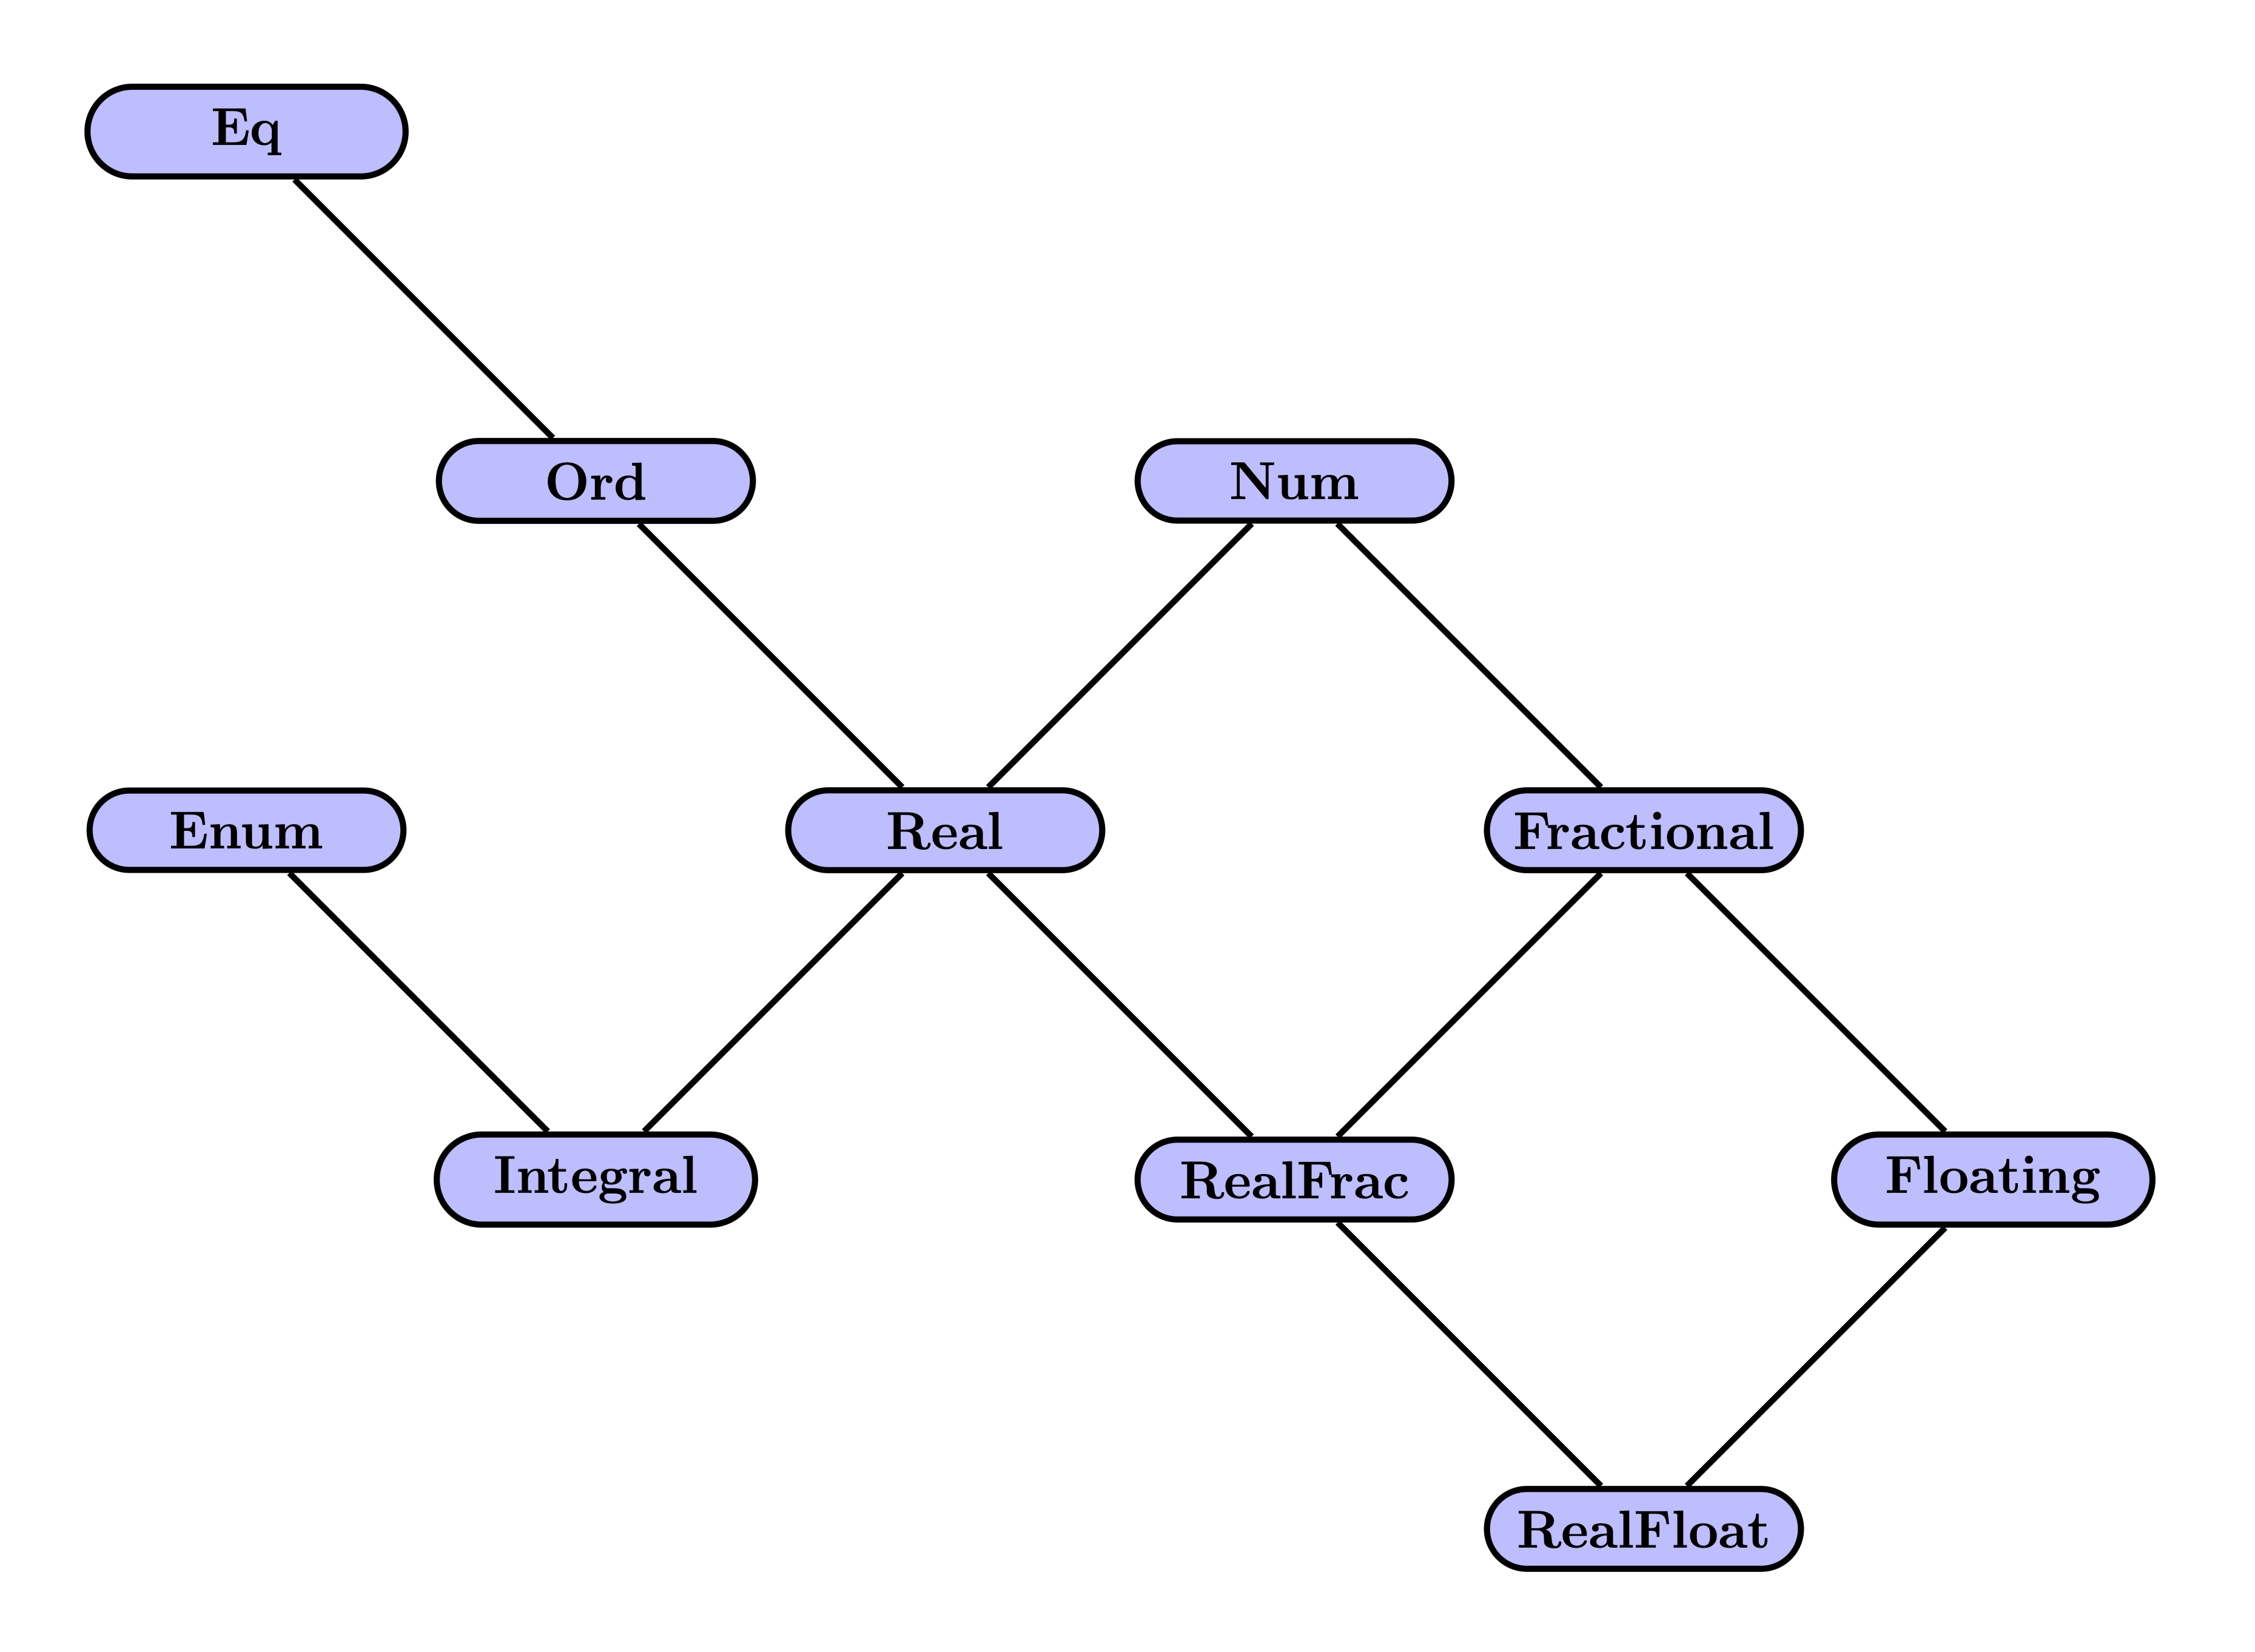
\includegraphics[width=8cm]{images/type-inclusion.png}
    \caption{Основни типови класове в Haskell [1]}
  \end{figure}

\end{frame}

\begin{frame}[fragile]
  \frametitle{Типови класове и типови променливи}

  \begin{tabular}{c|l}
    Eq & ==, /= \\
    Ord & <, <=, >, >= \\
    Show & show \\
    Read & read \\
    Num & +, -, *, abs, signum \\
    Integral & div, mod, toInteger \\
    Fractional & /, recip    
  \end{tabular}

  \bigskip

  \begin{itemize}
    \item Типови променливи
  \end{itemize}

\end{frame}

\begin{frame}[fragile]
  \frametitle{Произведение на типове}

  \begin{itemize}
    \item Двойки и n-торки
    \item \verb#fst, snd#
  \end{itemize}

\end{frame}


\subsection{Списъци и символни низове}

\begin{frame}
  \centerline{Списъци и символни низове}
\end{frame}
  
\begin{frame}[fragile]
  \frametitle{Списъци}

  \begin{itemize}
    \item Хомогенни линейни структури, \verb|[a]|
    \item Представяне в паметта
    \item Основни операции
  \end{itemize}

  \bigskip

  head, tail, last, init, length, null, reverse, take, drop, maximum, minimum, sum, product, elem

  \bigskip

  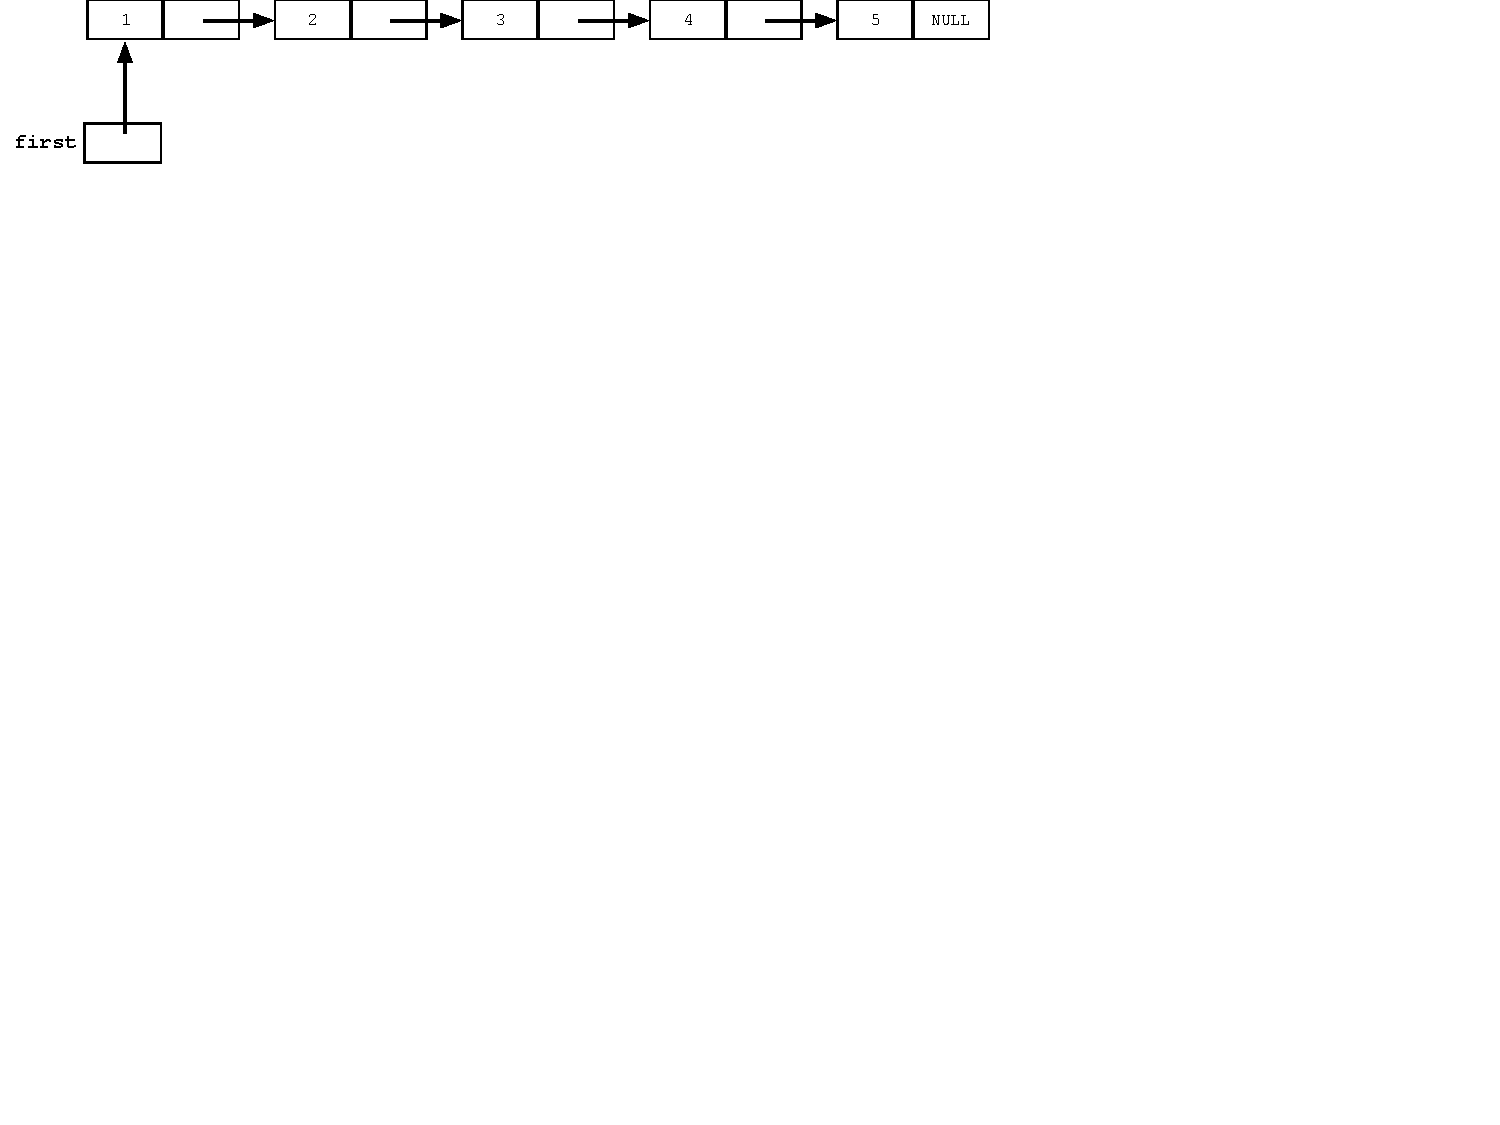
\includegraphics[width=14.0cm]{images/02_ll_flatchain}

\end{frame}


\begin{frame}[fragile]
  \frametitle{Оператори над списъци}

  \begin{itemize}
    \item Списъчен конструктор \verb|:|
    \item \verb|++|
    \item \verb|!!|
    \item Интервали
  \end{itemize}

  \bigskip

  head, tail, last, init, length, null, reverse, take, drop, maximum, minimum, sum, product, elem

\end{frame}

\begin{frame}[fragile]
  \frametitle{Операции със}

  \begin{itemize}
    \item zip и zipWith
  \end{itemize}

  \bigskip

  head, tail, last, init, length, null, reverse, take, drop, maximum, minimum, sum, product, elem

\end{frame}


\begin{frame}[fragile]
  \frametitle{Символни низове}

  \begin{itemize}
    \item Списъци от символи
  \end{itemize}

  \bigskip
  

\end{frame}



\subsection{}


\begin{frame}[fragile]
  \frametitle{Характеристика на езика}
  
\begin{itemize}
  \item Чисто функционален език
  \item Строго типизиран език
  \begin{lstlisting}[basicstyle=\small, language=Haskell]
    5 + "5"
    f :: [Int] -> Int
    f [] = 0
    f _ = 1
    \end{lstlisting}
  \item Лениво (мързеливо) оценяване
  \begin{lstlisting}[basicstyle=\small, language=Haskell]
    f x = x : f (x+1)
    take 5 (f 0)
  \end{lstlisting}
\end{itemize}


\end{frame}


\begin{frame}[fragile]
  \frametitle{Цитирани източници}

  \relscale{0.5}
    [1] Antoni Diller, Introduction to Haskell, 
        https://www.cantab.net/users/antoni.diller/haskell/haskell.html
\end{frame}


\begin{frame}[fragile]
    \frametitle{}
  
  \centerline{Благодаря за вниманието!}
\newcommand{\license}[1]{
  \begin{tikzpicture}[remember picture,overlay]
      \node[xshift=0mm,yshift=13mm,anchor=south east] at (current page.south east)
      {\tiny{Материалите са разработени от Калин Георгиев за курсовете по програмиране на ФМИ, СУ}};
      \node[xshift=0mm,yshift=10mm,anchor=south east] at (current page.south east)
      {\tiny{Creative Commons Attribution-NonCommercial-ShareAlike 4.0 International}};
      \node[xshift=0mm,yshift=5mm,anchor=south east] at (current page.south east){%
      \includegraphics[width=30mm]{{#1}/license}};
    \end{tikzpicture}
}
\license{../../..}
 
\end{frame}  


\end{document}
 


\begin{columns}[t]
  \begin{column}{0.2\textwidth}

\relscale{0.63}
\begin{lstlisting}
\end{lstlisting}
\relscale{1}

  \end{column}
  \begin{column}{0.8\textwidth}

  \end{column}
\end{columns}


